\section{TiXmlOutStream Class Reference}
\label{classTiXmlOutStream}\index{TiXmlOutStream@{TiXmlOutStream}}
{\tt \#include $<$tinystr.h$>$}

Inheritance diagram for TiXmlOutStream::\begin{figure}[H]
\begin{center}
\leavevmode
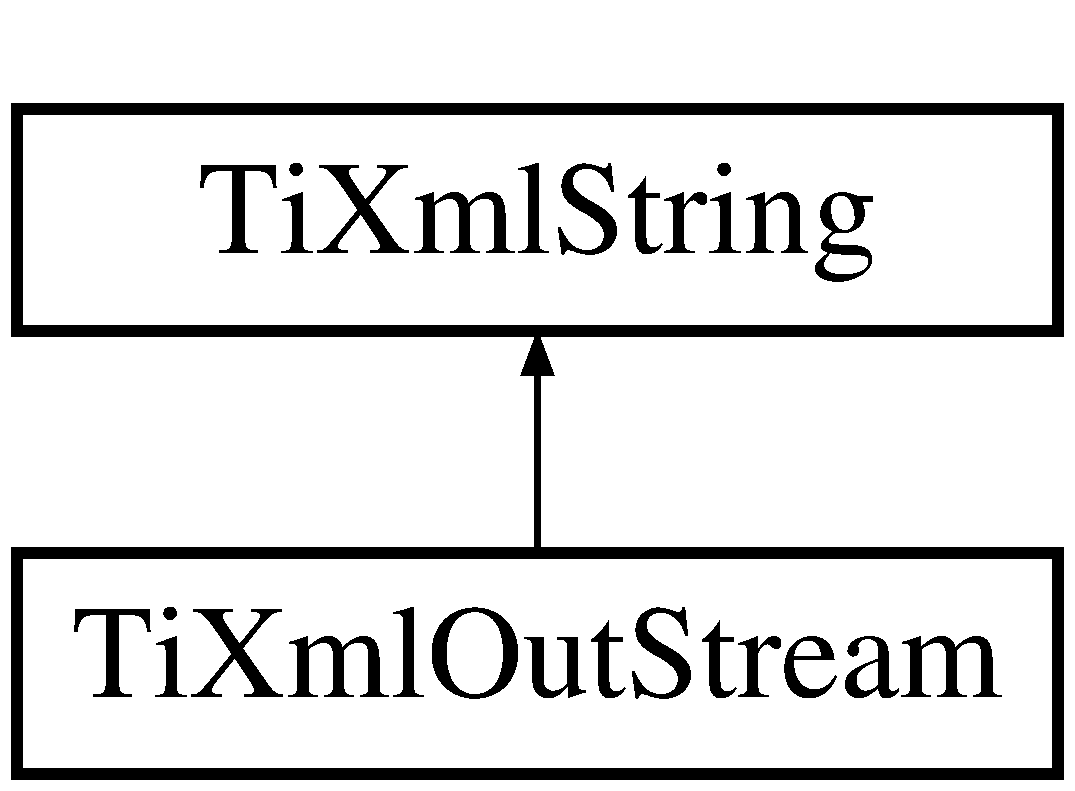
\includegraphics[height=2cm]{classTiXmlOutStream}
\end{center}
\end{figure}
\subsection*{Public Member Functions}
\begin{CompactItemize}
\item 
{\bf TiXmlOutStream} \& {\bf operator$<$$<$} (const {\bf TiXmlString} \&in)
\item 
{\bf TiXmlOutStream} \& {\bf operator$<$$<$} (const char $\ast$in)
\end{CompactItemize}


\subsection{Member Function Documentation}
\index{TiXmlOutStream@{TiXmlOutStream}!operator$<$$<$@{operator$<$$<$}}
\index{operator$<$$<$@{operator$<$$<$}!TiXmlOutStream@{TiXmlOutStream}}
\subsubsection[operator$<$$<$]{\setlength{\rightskip}{0pt plus 5cm}{\bf TiXmlOutStream}\& TiXmlOutStream::operator$<$$<$ (const {\bf TiXmlString} \& {\em in})\hspace{0.3cm}{\tt  [inline]}}\label{classTiXmlOutStream_3640dcb1c0903be3bc6966cdc9a79db6}


\index{TiXmlOutStream@{TiXmlOutStream}!operator$<$$<$@{operator$<$$<$}}
\index{operator$<$$<$@{operator$<$$<$}!TiXmlOutStream@{TiXmlOutStream}}
\subsubsection[operator$<$$<$]{\setlength{\rightskip}{0pt plus 5cm}{\bf TiXmlOutStream}\& TiXmlOutStream::operator$<$$<$ (const char $\ast$ {\em in})\hspace{0.3cm}{\tt  [inline]}}\label{classTiXmlOutStream_f2117e5a8cbfcb69544804ad2859bfb6}




The documentation for this class was generated from the following file:\begin{CompactItemize}
\item 
{\bf tinystr.h}\end{CompactItemize}
